%%%%%%%%%%%%%%%%%%%%%%%%%%%%%%%% 
\section{The Fine-Grained Tracker} 
\label{cdrsec:detectors-nd-ref}

The scope of the DUNE Fine-Grained Tracker (FGT) near neutrino
detector includes the design, procurement, fabrication, testing,
delivery and installation of all FGT subsystems:
\begin{itemize}
\item Central straw-tube tracker (STT)
\item Electromagnetic calorimeter (ECAL) 
\item Dipole magnet (0.4-T) surrounding the STT and ECAL
\item Muon identifiers (MuID): in the magnet steel and upstream/downstream of the STT
\item Instrumentation for monitoring and control
\end{itemize}



A schematic drawing of the FGT design is shown in Figure~\ref{fig:STT_schematic}. 
\begin{cdrfigure}[A schematic drawing of the fine-grained
tracker design]{STT_schematic}{A schematic drawing of the fine-grained tracker design.}
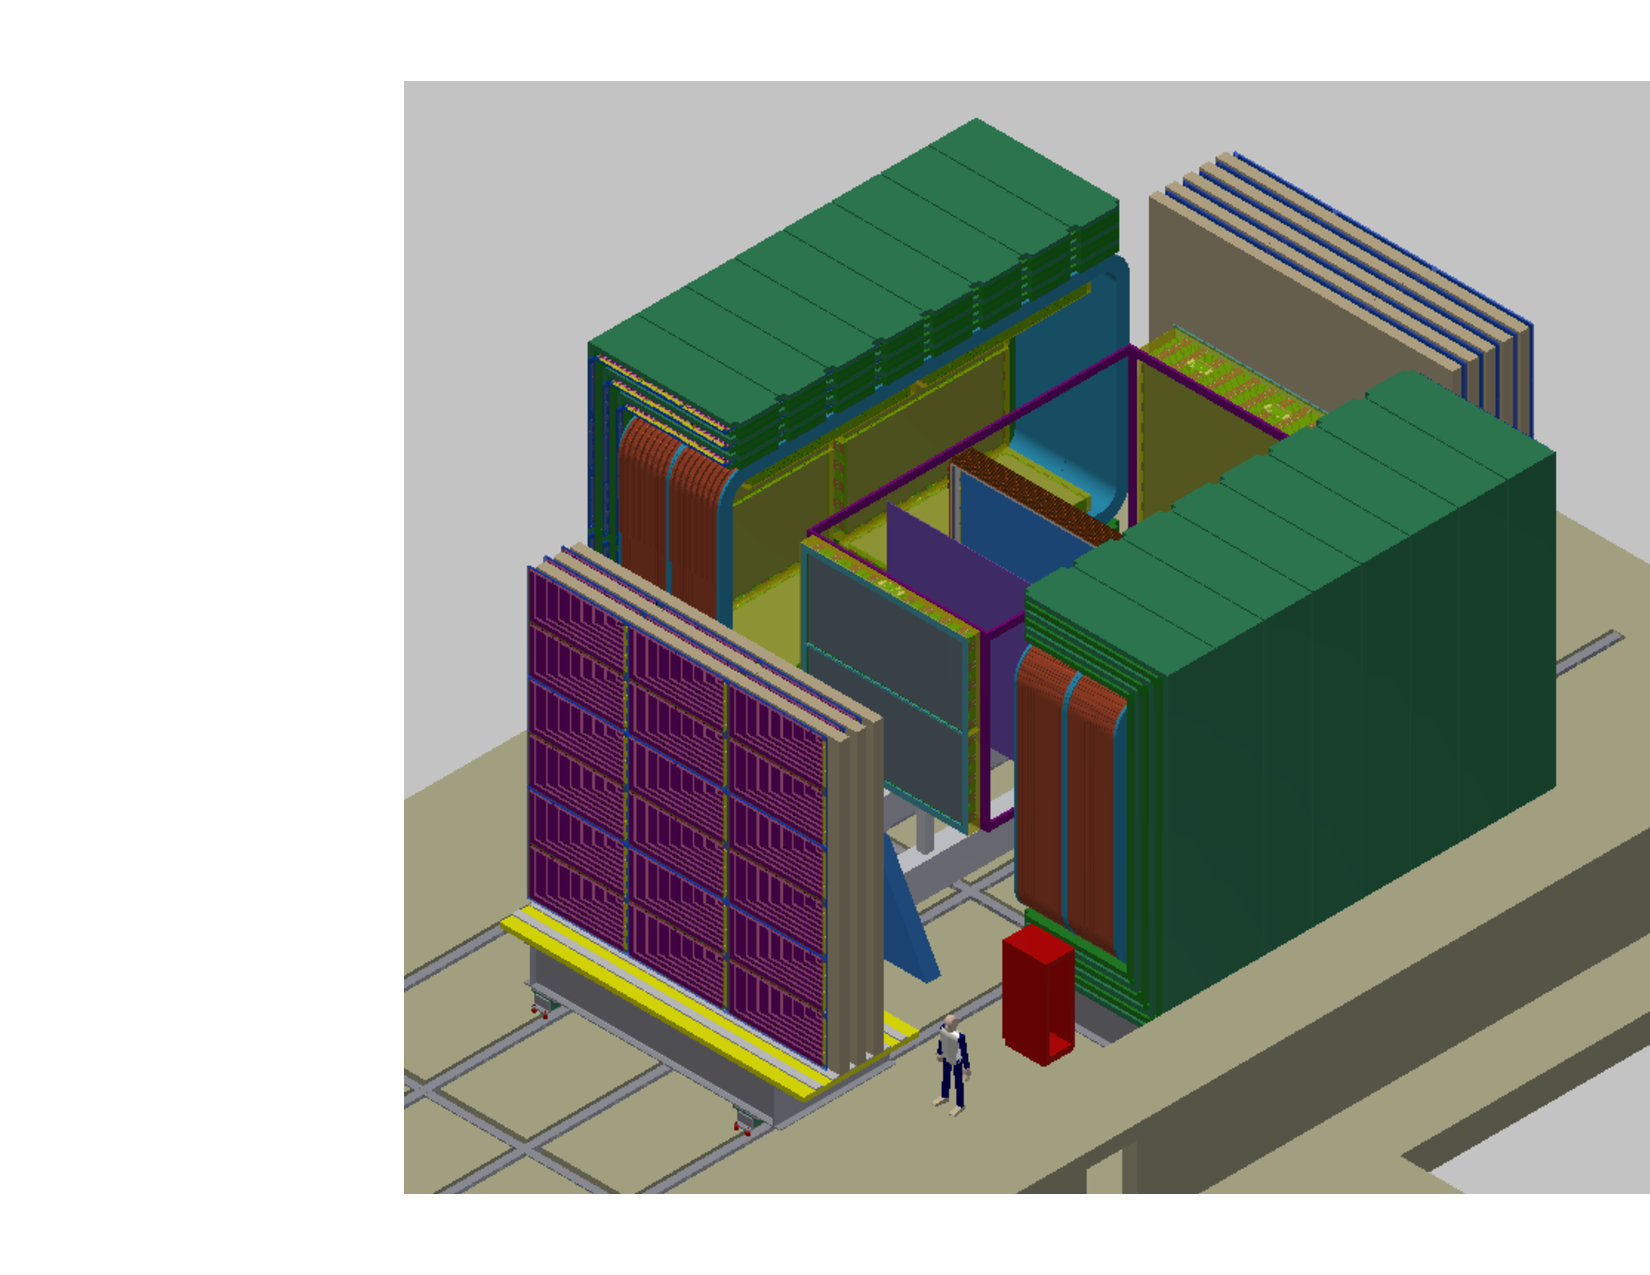
\includegraphics[width=0.8\textwidth]{FGT_Overview}
\end{cdrfigure}
The design presented here meets the required performance for making precision measurements of 
neutrino fluxes, cross sections, signal and background rates for the DUNE far detector. 
The DUNE ND is designed to fulfill the physics program described in Chapter 6 of CDR \volphys %Section~\ref{ch:physics-nd}, 
as well as the DAE/DST Detailed Project Report\cite{DPR}. The most significant 
requirements\cite{ND-REQ1,ND-REQ2} for the FGT include:  
\begin{itemize}
\item Muon energy scale uncertainty better than 0.2\% and hadronic
  energy scale uncertainty better than 0.5\% for the low-$\nu$ flux
  measurements
\item Magnetized detector capable of separating $\mu^+$
  from $\mu^-$, as well as $h^+$ from $h^-$, where $h$ is a charged
  hadron
\item Capability to to separate $e^+$ from $e^-$ for absolute and
  relative flux measurements
%\item low density $\rho \sim 0.1$ g/cm$^3$, similar to that of liquid hydrogen
%\item dipole magnetic field of $B=0.4$ T with high detector granularity 
\item Excellent momentum ($<5\%$) and angular ($<2$ mrad) resolutions
  for $\mu^{\pm}$, $e^{\pm}$, $\pi^{\pm}$ and proton, and
  $\pi^0$/$\gamma$ via decay/conversion, and $K^0_S$/$\Lambda$
  produced in $\nu$-induced interactions.
\item 4$\pi$ ECAL coverage to ensure an accurate determination of the
  momentum vector of the hadronic shower
\item 4$\pi$ MuID coverage to identify muons with a wide range of
  energies and angles
\item Electron/positron identification through the use of transition
  radiation (TR) in the entire tracking detector for low-energy and/or
  large angle tracks (e.g. $\gamma$ conversions)
\item $\pi/K/p$ identification by dE/dx in the entire tracking
  detector
\item Identification of $\pi^0$ and $\gamma$ that can mimic
  $\nu_e$ signals at the far detector
\item Use of a variety of nuclear targets, (C$_3$H$_6$)$_n$, Ar, Ca,
  C, Fe, etc., to quantify the impact of nuclear effects in
  $\nu$($\bar \nu$)-nucleus cross sections
\item Provide more than 10 times the unoscillated statistics on Ar targets expected
  in a 40-kt far detector
%\item  identification and measurement of processes such as neutral current $\pi^0$ production that can mimic oscillation signals at the FD
%\item comparability with measurements made in the FD
%\item measurement of nuclear effects, including short-range correlations, two-body currents, pion absorption, initial-state interactions, 
%and final-state interactions
\end{itemize}
The requirements listed above imply the use of a low density, $\rho
\sim$0.1~g/cm$^3$, high-resolution magnetic spectrometer.  A summary
of the performance requirements is given in Table~\ref{tab:comparison}
Regardless of the process under study, the goal is to have the
systematic error less than the corresponding statistical error.
\begin{cdrtable}[A summary of the performance for 
the FGT configuration]{ll}{comparison}{A summary of the performance for 
the FGT configuration}
Performance Metric&FGT\\ \toprowrule
Dipole magnetic field & 0.4 T \\ \colhline 
Average target/tracker density & $\rho \sim 0.1$ g/cm$^3$ \\ \colhline 
Target/tracker Volume & 3.5m x 3.5m x 6.4m \\ \colhline
Target/tracker Mass&8~t \\ \colhline
Vertex Resolution&0.1 mm \\ \colhline
Angular Resolution&2 mrad \\ \colhline
$E_e$ Resolution&5\% \\ \colhline
$E_\mu$ Resolution&5\% \\ \colhline
$\nu_\mu/\bar \nu_\mu$ ID&Yes \\ \colhline
$\nu_e/\bar \nu_e$ ID&Yes \\ \colhline
NC$\pi^0$/CCe Rejection&0.1\% \\ \colhline
NC$\gamma$/CCe Rejection&0.2\% \\ \colhline
CC$\mu$/CCe Rejection&0.01\% \\
\end{cdrtable}


%The FGT will measure the neutrino event rates and cross sections 
%on argon, water, and other nuclear 
%targets for both $\nu_e$ and $\nu_\mu$ charged current (CC) and
%neutral current (NC) scattering events. The FGT design 
%consists of a straw-tube tracker (STT), consisting of straw tubes, water targets, argon targets, 
%and radiator targets, and an electromagnetic calorimeter (ECAL), both inside a
%dipole magnet. In addition, muon detectors (MuID) consisting of resistive plate
%chambers (RPCs) will be embedded in the steel
%of the magnet. 



%%%%%%%%%%%%%%%%% 
\subsection{Straw-Tube Tracking Detector}
\label{cdrsec:detectors-nd-ref-fgt-stt}


\subsubsection{Straw Tubes} 

The Straw-Tube Tracking Detector (STT) at the center of the FGT 
is composed of straw tubes with an outer diameter of 1~cm, as well as 
radiators and targets that reside next to the straw tubes as shown in Figure~\ref{fig:STT_Detail}.
\begin{cdrfigure}[A schematic drawing of the straw tube tracker]
{STT_Detail}{A schematic drawing of the Straw-Tube Tracking Detector (STT) design.}
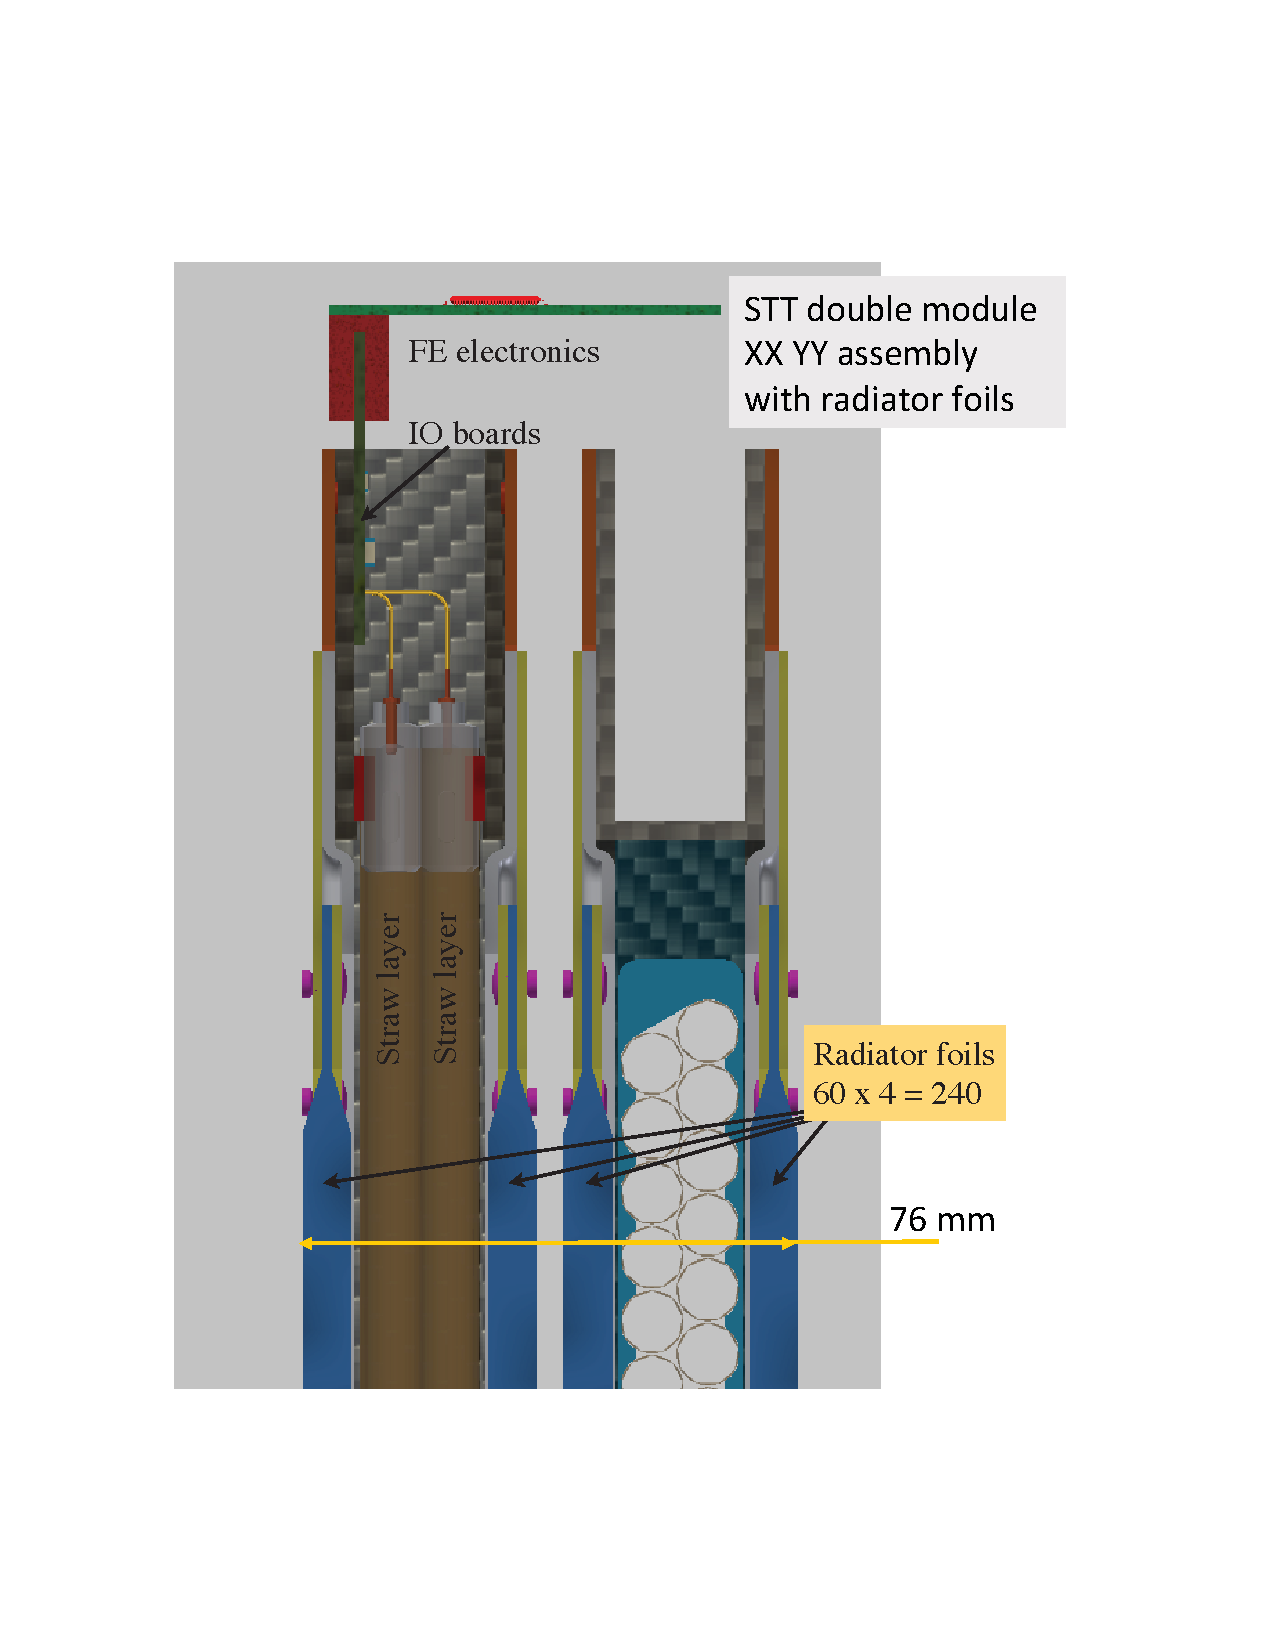
\includegraphics[width=0.4\textwidth]{STT_Detail}
\end{cdrfigure}

The straw walls are made by winding together a film of carbon loaded
Kapton XC (inner) and a film of aluminum coated Kapton HN (outer), for
a total thickness of about 70~$\mu$m. The anode wire will be gold plated 
tungsten with 20 $\mu m$ diameter. Vertical (YY) and horizontal
(XX) planes of straws will alternate and be arranged in modules, with
each module containing close-packed double straw layers of vertical
and horizontal straws (XXYY).  Figure~\ref{fig:STT_Detail} shows a
schematic drawing of an STT module with four straw-tube planes and
radiators. Each XXYY module equipped with radiators is equivalent to
$1.25 \times 10^{-2} X_0$, with a radiation length $X_0\sim$6~m. The
momentum measurement requires that tracks are detected in at least 6
straw layers. The staggered double layer design, high 
number of straw planes and the double-end readout
will contribute to the short track disambiguation.


The straw tubes will be filled with a gas mixture of either 70\% Ar
plus 30\% CO$_2$ (for modules with targets) or 70\% Xe plus 30\%
CO$_2$ (for modules with radiators).  The dimensions of each module in
the reference design will be approximately
350~cm$\times$350~cm$\times$ 8.0~cm, including target or radiator
planes and four straw planes. For ease of construction and
transportation, each module is made up of four sub-modules, with
dimensions of appproximately 350~cm$\times$175~cm$\times$4.0~cm.
%The straw tubes in a single sub-module will be able to provide the tension 
%for the wires, however, a temporary sub-module carbon composite frame will 
%be employed for shipping. 
The sub-modules will be assembled %put together into modules 
at Fermilab, where each module will have a carbon composite frame around 
the perimeter for support and will have an attached target or 
radiator. 
%Nominally, there will be 34 modules with targets and 46 modules 
%with radiators, still keeping the 
%average density of the STT at around 0.1 g/cm$^3$. 

The modularity of the STT provides for successive measurements using
thin nuclear targets (thickness $< 0.1 X_0$), while the excellent
angular and spatial resolution allows a clean separation of events
originating in different target materials.

The STT will have a total of 107,520 straws --- corresponding to 336
straws per plane, 1344 straws per module --- and 80 modules. Both ends
of the straw tubes will be read out, leading to a total number of
215,040 electronics channels. The total mass of the STT, including
targets and radiators, is approximately 8~t. Table~\ref{tab:STT_details} 
summarizes the main STT parameters.
\begin{cdrtable}[Straw Tube Detector specifications]{ll}{STT_details}{Straw Tube Detector specifications}
Item&Specification \\ \toprowrule
Straw Tube Geometry & 1cm Diameter x 3.5m Long \\ \colhline
Number of Straw Tubes & 107,520 \\ \colhline
Number of Straw Tubes per Plane & 336 \\ \colhline
Number of Straw Tube Planes per Module & 4 \\ \colhline
Number of Straw Tube Sub-Modules per Module & 4 \\ \colhline
Number of Straw Tube Modules & 80 \\ \colhline
Number of Straw Tube Sub-Modules & 320 \\ \colhline
Length of Straw Tube Wire & 376.3 km \\ \colhline
Number of Electronics Channels & 215,040 \\ \colhline
Number of Modules with Radiators & 70 \\ \colhline
Radiator Thickness per Module & 3.6cm \\ \colhline
Radiator Mass per Module & 69.1 kg \\ \colhline
Number of Modules with Nuclear Targets & 10 \\ \colhline
C Mass per Target Plane & 192 kg \\ \colhline  
Number of Modules with C Target Planes & 2 \\ \colhline 
Ca Mass per Target Plane & 132 kg \\ \colhline  
Number of Modules with Ca Target Planes & 1 \\ \colhline 
Ar Target Geometry & 1.27cm Diameter $\times$ 3.5m long \\ \colhline
Number of Ar Targets per Plane & 275 \\ \colhline
Ar Mass per Target Plane & 15.5 kg \\ \colhline  
Number of Modules with Ar Target Planes & 6 \\ \colhline
Fe Mass per Target Plane & 96.5 kg \\ \colhline  
Number of Modules with Fe Target Planes & 1 \\  
%Water Mass per Target Plane & 95 kg \\
\end{cdrtable}
In addition to tracking charged particles and measuring Transition Radiation (TR), 
the STT provides dE/dx measurement to identify particles. 
Figure~\ref{fig:PartID_dedx} provides a sample of pions, kaons and protons identified via dE/dx in the STT.
\begin{cdrfigure}[Simulated distributions of dE/dx for different particles in FGT]
{PartID_dedx}{Simulated distributions of dE/dx for different particles in FGT.}
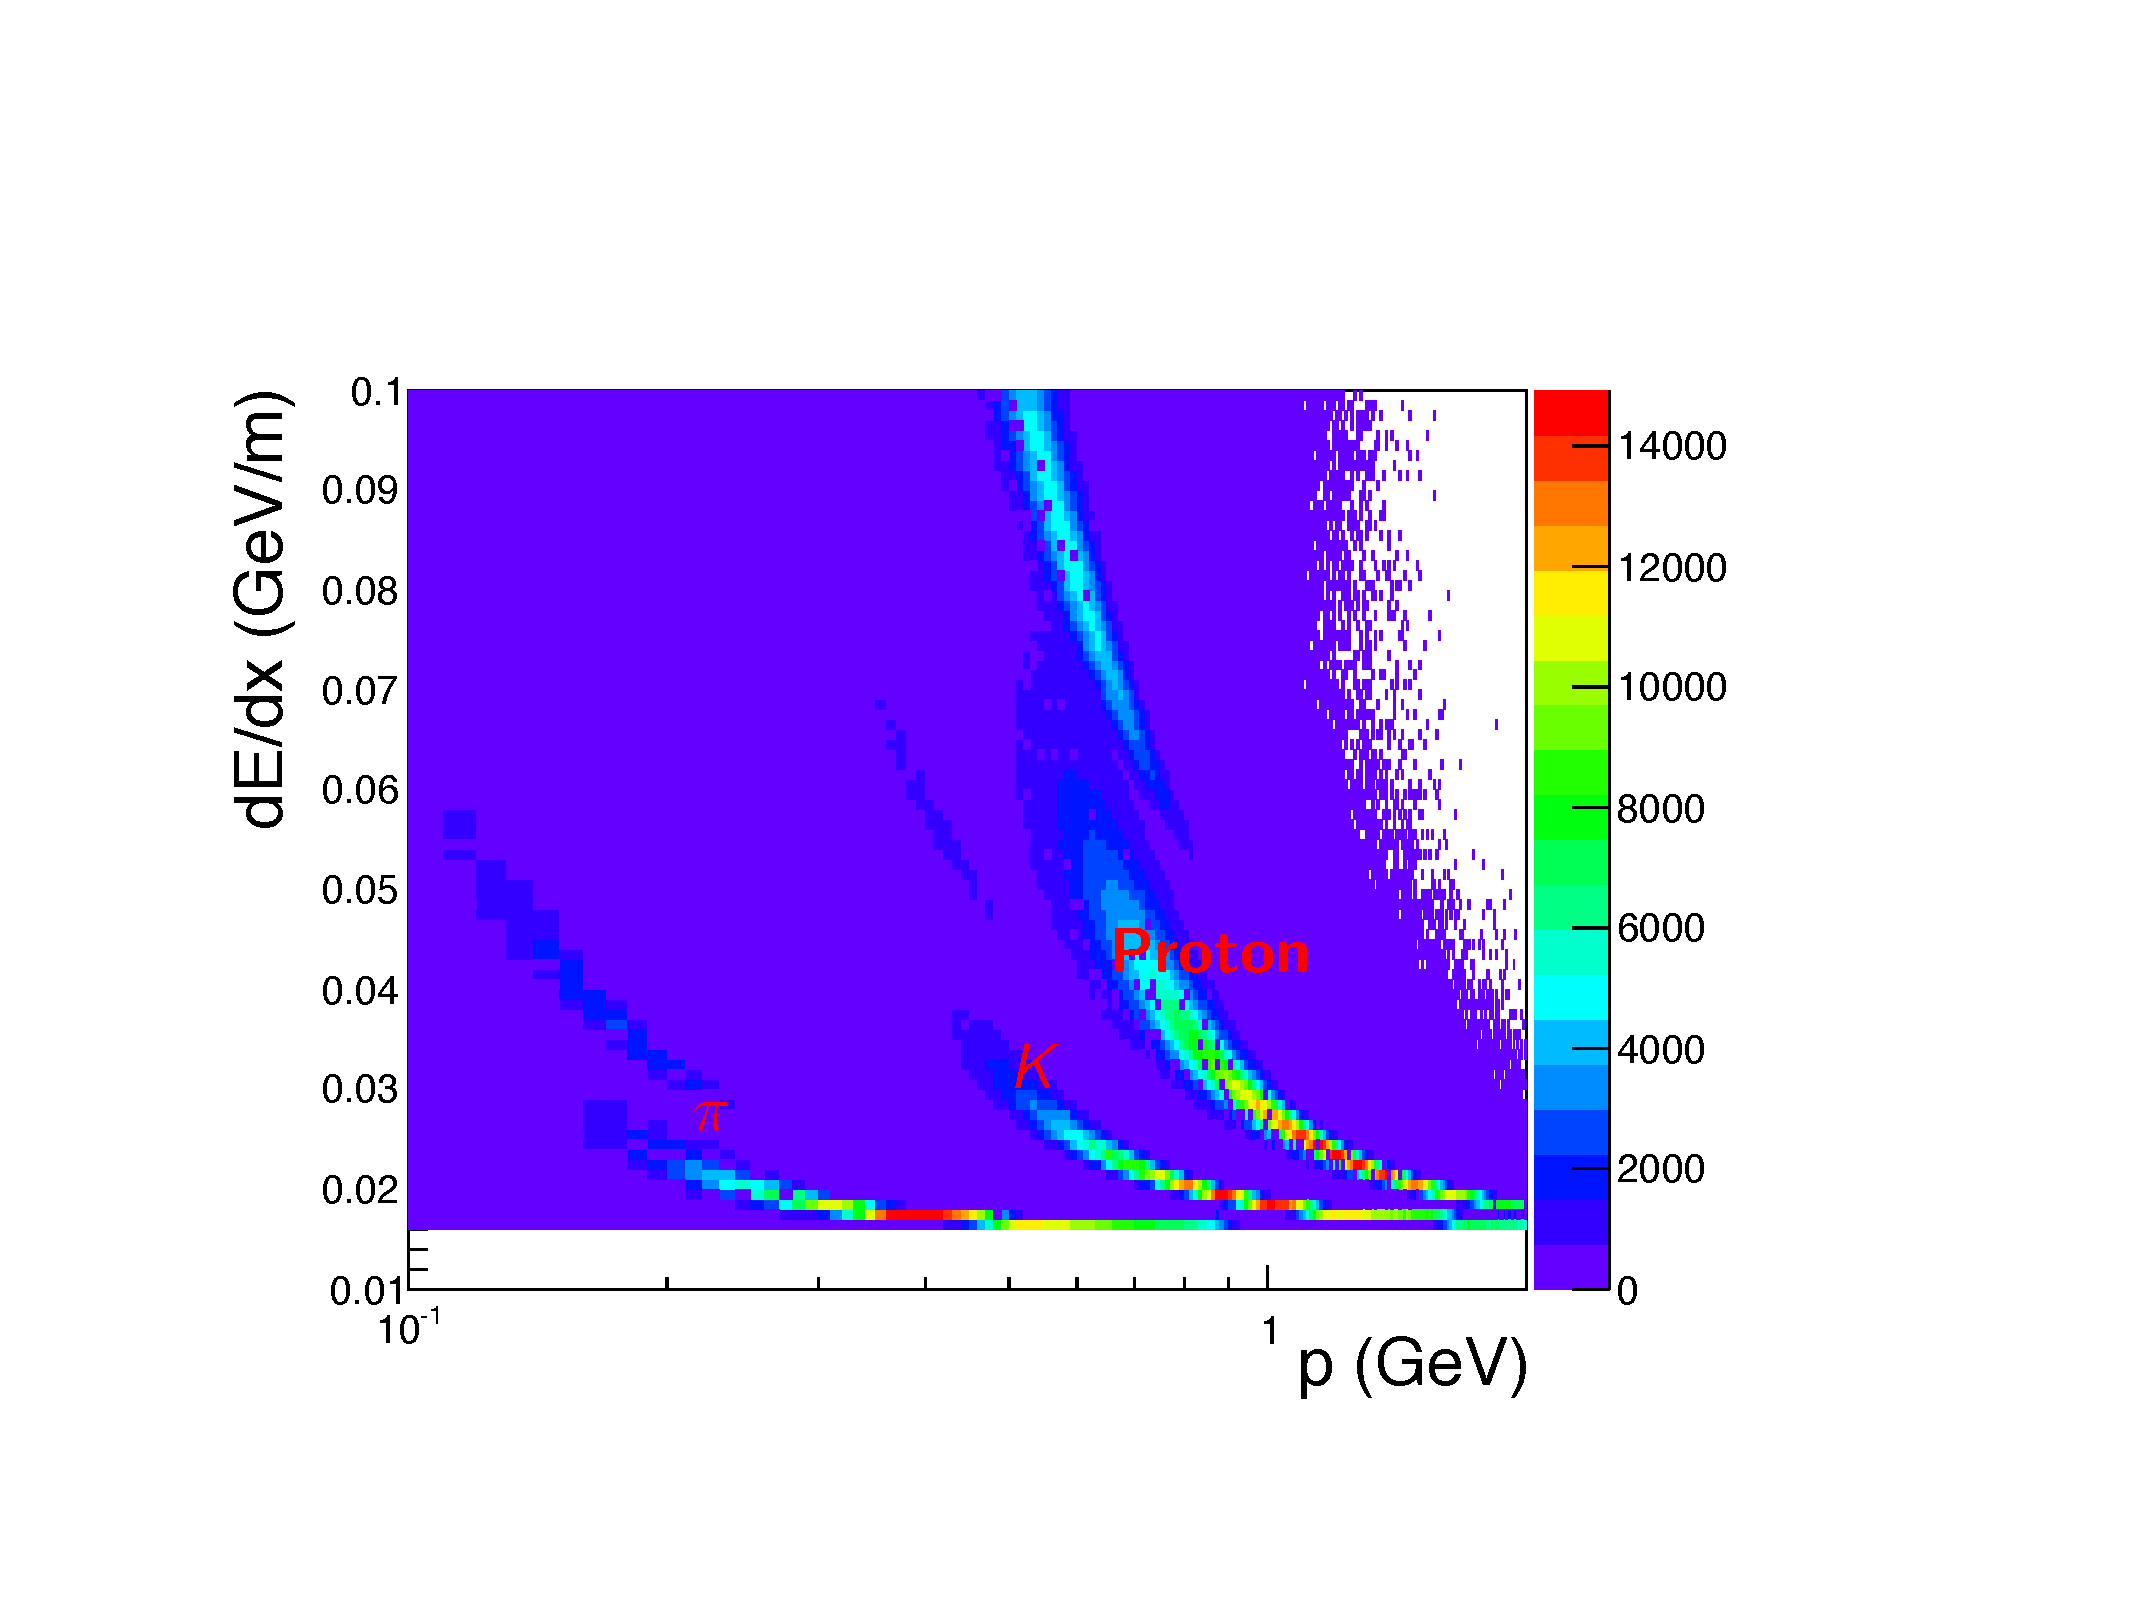
\includegraphics[width=0.7\textwidth]{PartID_dedx}
\end{cdrfigure}

\subsubsection{Radiator Targets} 


Radiators will be placed in the downstream STT modules and will serve
as targets for both neutrino interactions and Transition Radiation
(TR) production. Each STT module contains four radiators, where each
radiator consists of 60 layers of 25-$\mu$m polypropylene
(C$_3$H$_6$)$_n$ foils, which are embossed to keep 125-$\mu$m air gaps
between consecutive foils.  The mass of each radiator is $\sim$17~kg
and the thickness is $\sim$9~mm. The use of thin plastic foils
regularly spaced allows the emission of transition radiation for
electron/positron identification, which is detected by the Xe gas in
the straws. The plastic radiators account for about 83\% of the mass of each STT module and 
also provide the main (anti)neutrino target. Overall, a radiator mass of about 5 tons 
is required to achieve the physics sensitivity discussed in 
Chapter 6 of CDR \volphys %Section~\ref{ch:physics-nd} 
and the DAE/DST Detailed Project Report\cite{DPR}. 

\subsubsection{Nuclear Targets} 

A set of different nuclear targets will be installed in front of the
most upstream STT modules, which will not be equipped with radiators.
The most important nuclear target is the argon target that matches
the DUNE far detector.  This target will consist of planes of 0.5-inch
diameter, 3.5-m-long stainless steel tubes, with wall thickness 0.065-inch,
filled with argon gas pressurized to 140~atm ($\rho = 0.233$), with
sufficient Ar mass to provide $\sim$10 times the unoscillated
statistics expected in a 40~t far detector.  We are currently investigating the
possibility to use carbon-composite tubes instead of stainless steel to contain 
the pressurized Ar gas.

Relevant to argon, a crucial target is calcium which has the same
atomic weight ($A=40$) as argon but is isoscalar.  Since most nuclear
effects depend on the atomic weight $A$, inclusive properties of
(anti)neutrino interactions are expected to be the same for these two
targets.  This fact would allow the use of both targets to model
signal and backgrounds in the DUNE far detector (argon target), as
well as to compare DUNE results for nuclear effects on argon with the
extensive data on calcium from charged lepton scattering.


An equally important nuclear target is carbon (graphite), which is
essential in order to get (anti)neutrino interactions on free proton,
through a statistical subtraction procedure from the main
polypropylene target (C$_3$H$_6$)$_n$.  The availability of such a
free-proton target will allow accurate flux determinations and cross
section measurements, and, for the first time, a direct
model-independent measurement of nuclear effects --- including both
the primary and final-state interactions --- on the argon target
relevant for the far detector oscillation analysis. The required
carbon target mass is about 0.5~t (in addition to the carbon in the
STT frames). The corresponding expected number of events on H target
are $5.0 (1.5) \times 10^6 \pm 13(6.6) \times 10^3$ $\nu(\bar \nu)$
CC, where the uncertainty is dominated by the subtraction procedure.

A stainless steel target in the form of a single thin slab will
provide service measurements of (anti)neutrino cross-sections for the
INO experiment in India.

Finally, the same stainless steel tubes used for the pressurized Ar gas can
be filled with standard and heavy water (H$_2$O and D$_2$O). The
statistical subtraction of H$_2$O from D$_2$O would result in a
quasi-free neutron.

Table~\ref{tab:STT_details} gives a reference configuration of the
radiators and nuclear targets, listed according to their location from
downstream to upstream.  The final configuartion of the nuclear
targets will require detailed Geant4 simulations of FGT and
corresonding physics sensitivity studies.


%%%%%%%%%%%%%%%%% 
\subsection{Electromagnetic Calorimeter}
\label{cdrsec:detectors-nd-ref-fgt-ecal}

An electromagnetic calorimeter (ECAL) will surround the tracking
volume on all sides and consist of three separate pieces: Forward
ECAL, Barrel ECAL and Backward ECAL.  The expected energy resolution
is $\sim 5\% / \sqrt{E}$ for the forward ECAL.  The ECAL must provide
high segmentation in both the transverse and longitudinal directions
to reconstruct photons from $\pi^0$ decay and electron/positrons from
their Bremsstrahlung emissions.  The ECAL conceptual design consists
of layers of either 1.75-mm-thick (for the forward ECAL) or
3.5-mm-thick (for the barrel and backward ECAL) lead sheets and
2.5-cm-wide by 10-mm-thick plastic scintillator bars, as shown in
Figure~\ref{fig:ECAL_detail}.
\begin{cdrfigure}[Schematic drawing of the ECAL]{ECAL_detail}
{Schematic drawing of the ECAL, which is made up of alternating planes
of plastic scintillator and Pb sheets.}
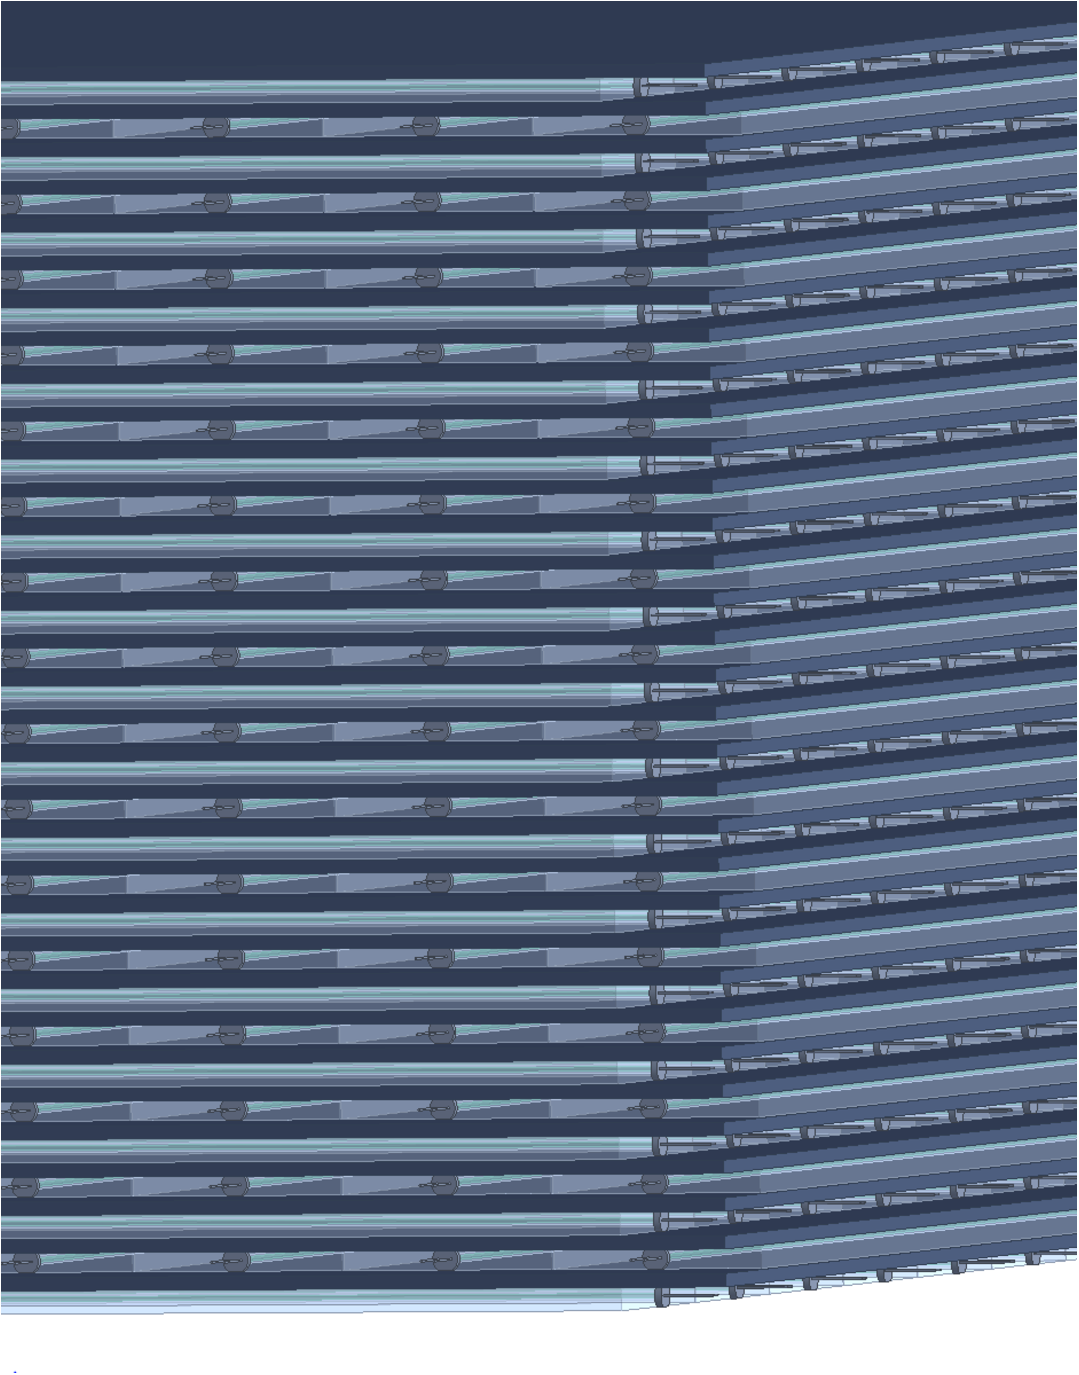
\includegraphics[width=0.4\textwidth,angle=0]{ECAL_detail}
\end{cdrfigure}
The scintillator layers for the Forward and Backward ECAL alternate as
XYXYXY..., while the scintillator layers for the Barrel ECAL are all
horizontal along the axis of the magnet.  The Forward ECAL will
consist of 60 layers of scintillator bars, where each bar has
dimensions 3.2~m$\times$2.5~cm$\times$1~cm. The Backward ECAL will
consist of 16 layers of scintillator bars, where each bar has the same
dimensions, 3.2~m$\times$2.5~cm$\times$1~cm. The Barrel ECAL will also
consist of 16 layers of scintillator bars, where each bar has the same
dimensions, 3.2~m$\times$2.5~cm$\times$1~cm. The parameters of the
ECAL design will be further optimized with the help of a full Geant
simulation of FGT.

The lead sheets and scintillator bars will be assembled and glued
together into complete modules of dimension
3.2~m$\times$3.2~cm$\times$81~cm for the Forward ECAL and
3.2~m$\times$3.2~cm$\times$27.5~cm for the Backward ECAL. For the
Barrel ECAL, the module dimensions will also be
3.2~m$\times$3.2~cm$\times$27.5~cm. Two Barrel modules are placed
end-to-end along the sides of the inner surface of the magnet (eight
Barrel modules total) to provide full coverage of the barrel region.
The total numbers of scintillator bars in the Forward (7680), Backward
(2048) and Barrel ECAL (16384) is 26112 bars.

The scintillator bars will be extruded with holes in the middle of
each bar. The holes will then be fitted with 0.7-mm-diameter Kuraray
wavelength-shifting (WLS) fibers.  The fibers will be read out by SiPM
(silicon photomultiplier) photosensors at each end.  Detailed R\&D
studies will be performed to optimize the diameter of the scintillator
hole, the fiber diameter and the proper coupling between the
scintillator and the fiber for optimum light transmission.


The total mass of scintillator is 20.9~t, the total mass of Pb is
70.8~t, and the total number of readout channels is 52,224.
Table~\ref{tab:ECAL_specs} summarizes the specifications of the ECAL.
\begin{cdrtable}[ECAL specifications]{ll}{ECAL_specs}{ECAL specifications}
Item&Specification \\ \toprowrule
Scintillator Bar Geometry & 3.2m $\times$ 2.5cm $\times$ 1cm \\ \colhline
Number of Forward ECAL Scintillator Bars & 7680 \\ \colhline
Forward ECAL Pb thickness & 1.75mm \\ \colhline
Number of Forward ECAL Layers & 60 \\ \colhline
Number of Forward ECAL Radiation Lengths & 20\\ \colhline
Dimensions of Forward ECAL Module & 3.2m $\times$ 3.2m $\times$ 81cm \\ \colhline
Number of Barrel ECAL Scintillator Bars & 16,384 \\ \colhline
Barrel ECAL Pb thickness & 3.5mm \\ \colhline
Number of Barrel ECAL Layers & 16 \\ \colhline
Number of Barrel ECAL Radiation Lengths & 10 \\ \colhline
Number of Barrel ECAL Modules & 8 \\ \colhline
Dimensions of Barrel ECAL Modules & 3.2m $\times$ 3.2m $\times$ 27.5cm \\ \colhline
Number of Backward ECAL Scintillator Bars & 2048 \\ \colhline
Backward ECAL Pb thickness & 3.5mm \\ \colhline
Number of Backward ECAL Layers & 16 \\ \colhline
Number of Backward ECAL Radiation Lengths & 10 \\ \colhline
Dimensions of Backward ECAL Module & 3.2m $\times$ 3.2m $\times$ 27.5cm \\ \colhline
Total Length of 0.7mm Diameter WLS Fiber & 83.6km \\ \colhline
Total Number of Scintillator Bars & 26,112 \\ \colhline
Total Number of Electronics Channels & 52,224\\ \colhline
Total Mass of Scintillator & 20,890 kg \\ \colhline
Total Mass of Pb & 70,800kg \\\end{cdrtable}




%%%%%%%%%%%%%%%%% 
\subsection{Dipole Magnet}
\label{cdrsec:detectors-nd-ref-fgt-magnet}

The STT and ECAL modules will reside inside a 0.4-T dipole magnet for
the measurement of particle momentum and charge.  The magnet will have
inner dimensions (inside the coils) 4.5-m wide $\times$ 4.5-m high
$\times$ 8.0-m long. The magnet has four vertical Al coils, stacked
horizontally, producing a horizontal magnetic field. The return yoke
will be divided into two halves along the longitudinal center line to
allow the magnet to be opened to service the detector inside. %, as
shown in Figure~\ref{fig:STT_schematic}.  Each half yoke will be built
from eight ``C'' (C-shaped) sections, and the thickness of the magnet
steel will be 60~cm, consisting of 6$\times$10-cm-thick plates. The
magnet power requirement with Al coils is $\sim$2.4~MW, corresponding
to 6~kA at 400~V. The water flow required for cooling is 20~l/s.
Figure~\ref{fig:Magnet_Bfield} shows the $B$ field results obtained
from detailed simulations performed at the Bhabha Atomic Research
Center (BARC) in India.
\begin{cdrfigure}[Magnetic field maps]{Magnet_Bfield}{Design of the dipole magnet and simulation of the 
corresponding magnetic field at the Bhabha Atomic Research Center (BARC) in India.}  
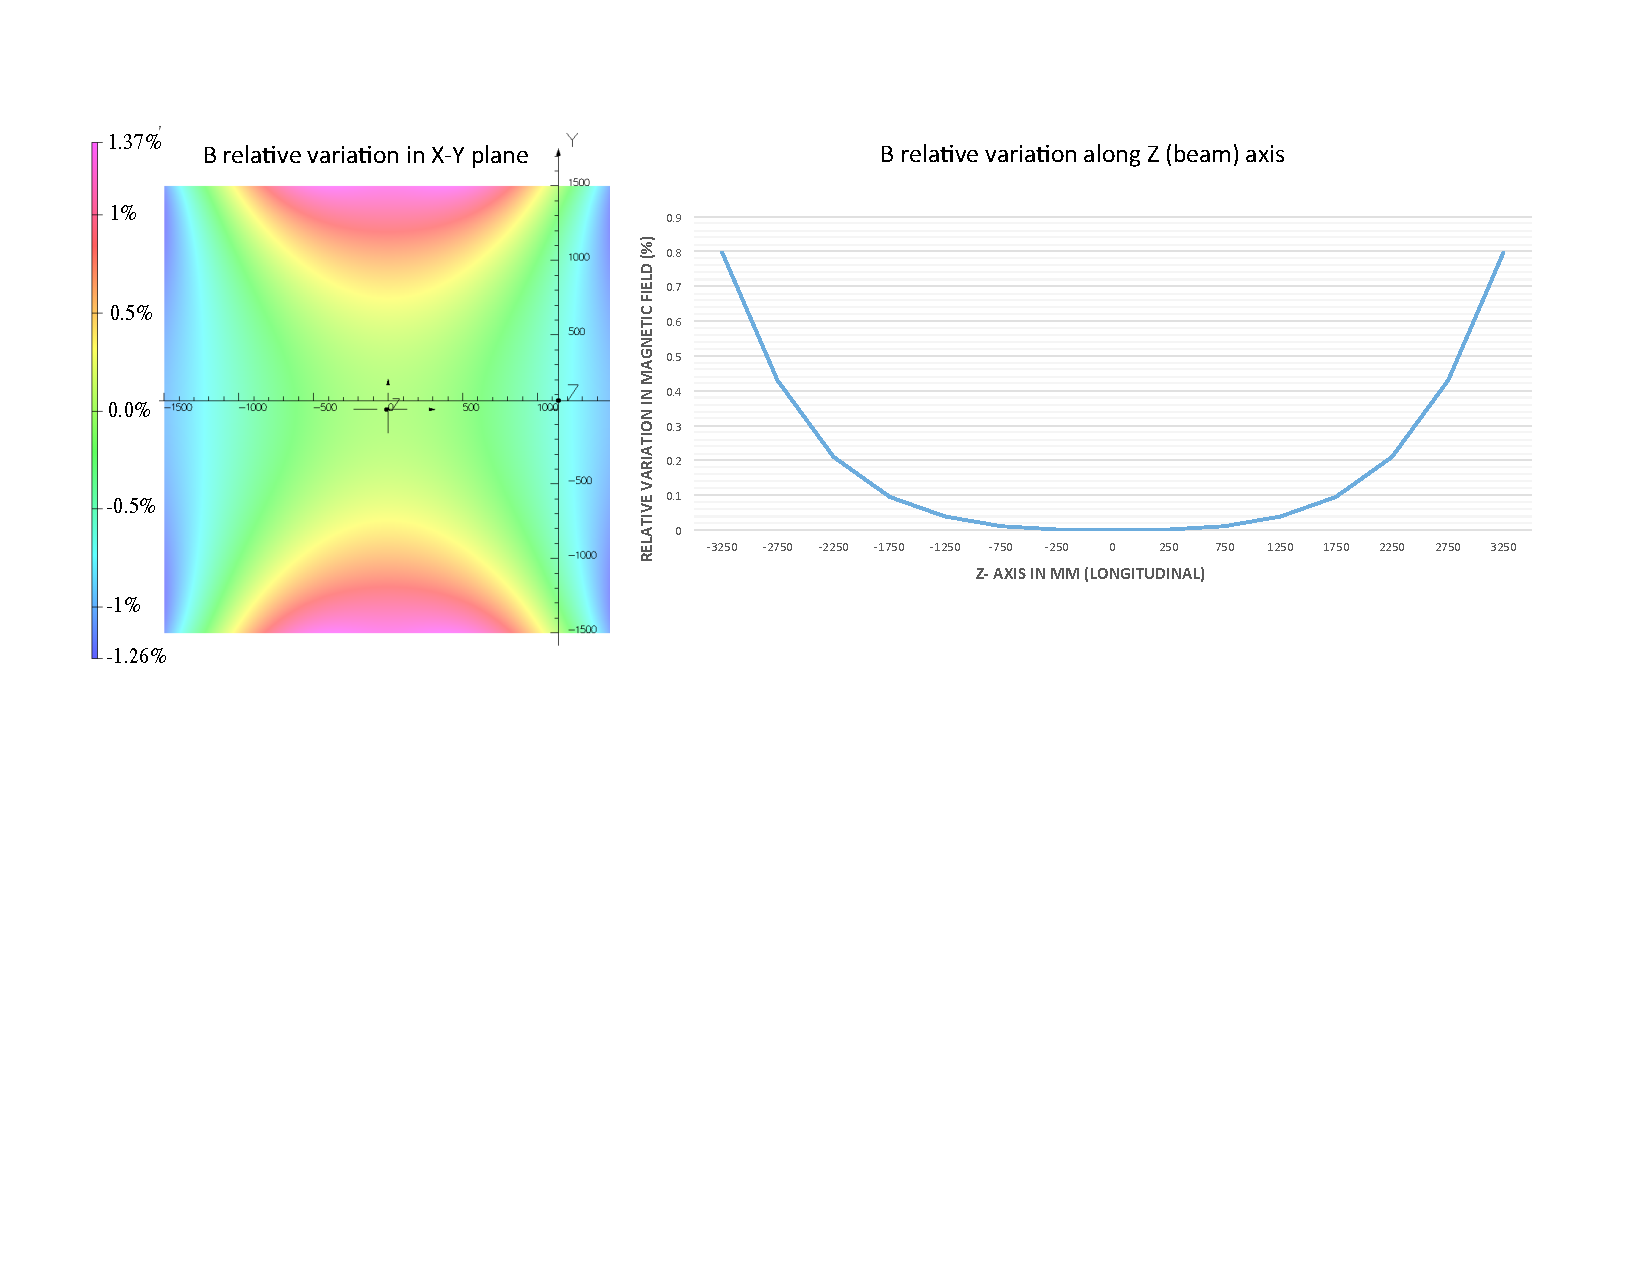
\includegraphics[width=\textwidth]{Magnet_Bfield} % [width=6in,angle=90] <-- was too small
\end{cdrfigure}
The magnet specifications are summarized in Table~\ref{tab:Magnet_specs}.
\begin{cdrtable}[Dipole Magnet specifications]{ll}{Magnet_specs}{Dipole Magnet specifications}
Item&Specification \\ \toprowrule
Inner Dimensions & 4.5m x 4.5m x 8.0m \\ \colhline
Magnetic Field & 0.4 T \\ \colhline
Number of ``C'' Sections & 16 \\ \colhline
Thickness of Steel in the ``C'' Sections & 60cm \\ \colhline
Mass per ``C'' Section & 60~t \\ \colhline
Number of Coils & 4 \\ \colhline
Mass per Coil & 40~t \\ \colhline
Magnet Current & 6 kA \\ \colhline
Magnet Voltage & 400 V \\ \colhline
Magnet Power Requirements & 2.4 MW \\ \colhline
Water Flow for Cooling & 20 l/s \\\end{cdrtable}


The momentum resolution is dominated by multiple scattering in the
STT. The momentum resolution is, therefore, given by $\delta p/p =
0.053/\sqrt(LX_0)B$. For B = 0.4T, L = 3m, and $X_0 = 4$m, the
expected momentum resolution is $\sim$3.8\%.

%%%%%%%%%%%%%%%%% 
\subsection{Muon Identifier}
\label{cdrsec:detectors-nd-ref-fgt-muonid}

The sides and ends of the dipole magnet will be instrumented with a
muon identifier detector (MuID) that will distinguish muons from
hadrons by the ability of muons to penetrate the iron without
showering or interacting.  The task of the MuID is to reconstruct the
muon track segments and match them with the corresponding charged
track reconstructed in the STT.  The MuID will consist of 432
resistive plate chamber (RPC) modules interspersed between two
10-cm-thick steel plates of the dipole magnet and between 20-cm-thick
steel plates at the upstream and downstream ends of the magnet as is
detailed in Table~\ref{tab:MID_specs}. 
\begin{cdrtable}[MuID specifications]{ll}{MID_specs}{MuID specifications}
Item&Specification  \\ \toprowrule
Number of Barrel RPC Trays of Dimension 2.2m $\times$ 4m & 8 \\ \colhline
Number of Barrel RPC Trays of Dimension 2.5m $\times$ 4m & 16 \\ \colhline
Number of Barrel RPC Trays of Dimension 2.8m $\times$ 4m & 16 \\ \colhline
Number of Barrel RPC Trays of Dimension 3.1m $\times$ 4m & 8 \\ \colhline
Number of END RPC Trays of Dimension 2m $\times$ 6m & 24 \\ \colhline
Total Number of RPC Trays & 72 \\ \colhline
Total Number of RPC Modules & 432 \\ \colhline
Mass of Downstream Steel Planes & 283,500 kg \\ \colhline
Mass of Upstream Steel Planes & 170,100 kg \\ \colhline
RPC Thickness & 1.5cm \\ \colhline
Number of 7.65mm Pitch X Strips per Module & 256 \\ \colhline
Number of 7.5mm Pitch Y Strips per Module & 128 \\ \colhline
Total Number of RPC Strips and Electronics & 165,888 \\
\end{cdrtable}
The choice of RPC is motivated by the combineation of low cost,
ability to reach sub-mm space resolution, and existing expertise.
The MuID is only meant to provide identification of the muon; the muon
momentum will be measured by the STT inside the magnetic field.



The nominal dimensions of all RPC modules will be 1~m $\times$ 2~m
with active areas of 96~cm $\times$ 196~cm. Each module has 256 X
strips at 7.65-mm pitch and 128 Y strips at 7.5-mm pitch. This
fine-grained pitch allows to reach spatial resolution of $\sim$0.7~mm
and to disentangle multiple hits resulting from events originated in
the magnet iron.  The modules will be grouped into trays, each
containing six modules, and the trays will be sufficiently wide to
allow overlapping modules.  The downstream MuID will contain five
steel planes of overall dimensions 6$\times$6$\times$0.2~m$^3$
(283.5~t) and five RPC planes, while the upstream MuID will contain
three steel planes (170.1~t) of dimensions 6$\times$6$\times$0.2~m$^3$
and three RPC planes. The barrel MuID will contain 24 planes (three
layers $\times$ eight sides) of RPCs. The RPCs will have a total
thickness of 15~mm and a gap width of 2~mm. One possible gas mixture
could be Ar (75\%), tetraflouroethane (20\%), isobutane (4\%) and
sulphurhexaflouride (1\%).  A full scale prototype of the RPC modules
was built at the Variable Energy Cyclotron Centre (VECC) in India.
Figure~\ref{fig:FGT_RPC} shows a picture taken during the assembly of
the prototype and the corresponding efficiency measurement with a
cosmic ray telescope.
%\begin{cdrfigure}[Schematic drawing of an RPC]{FGT_RPC}{Schematic drawing of an RPC.}
\begin{cdrfigure}[Fabrication and test of RPC prototype]{FGT_RPC}{Fabrication of a large 
(2.4~m$\times$1.2~m) RPC prototype at the Variable Energy Cyclotron Centre (VECC) in India 
(left) and corresponding efficiency tests (right).}
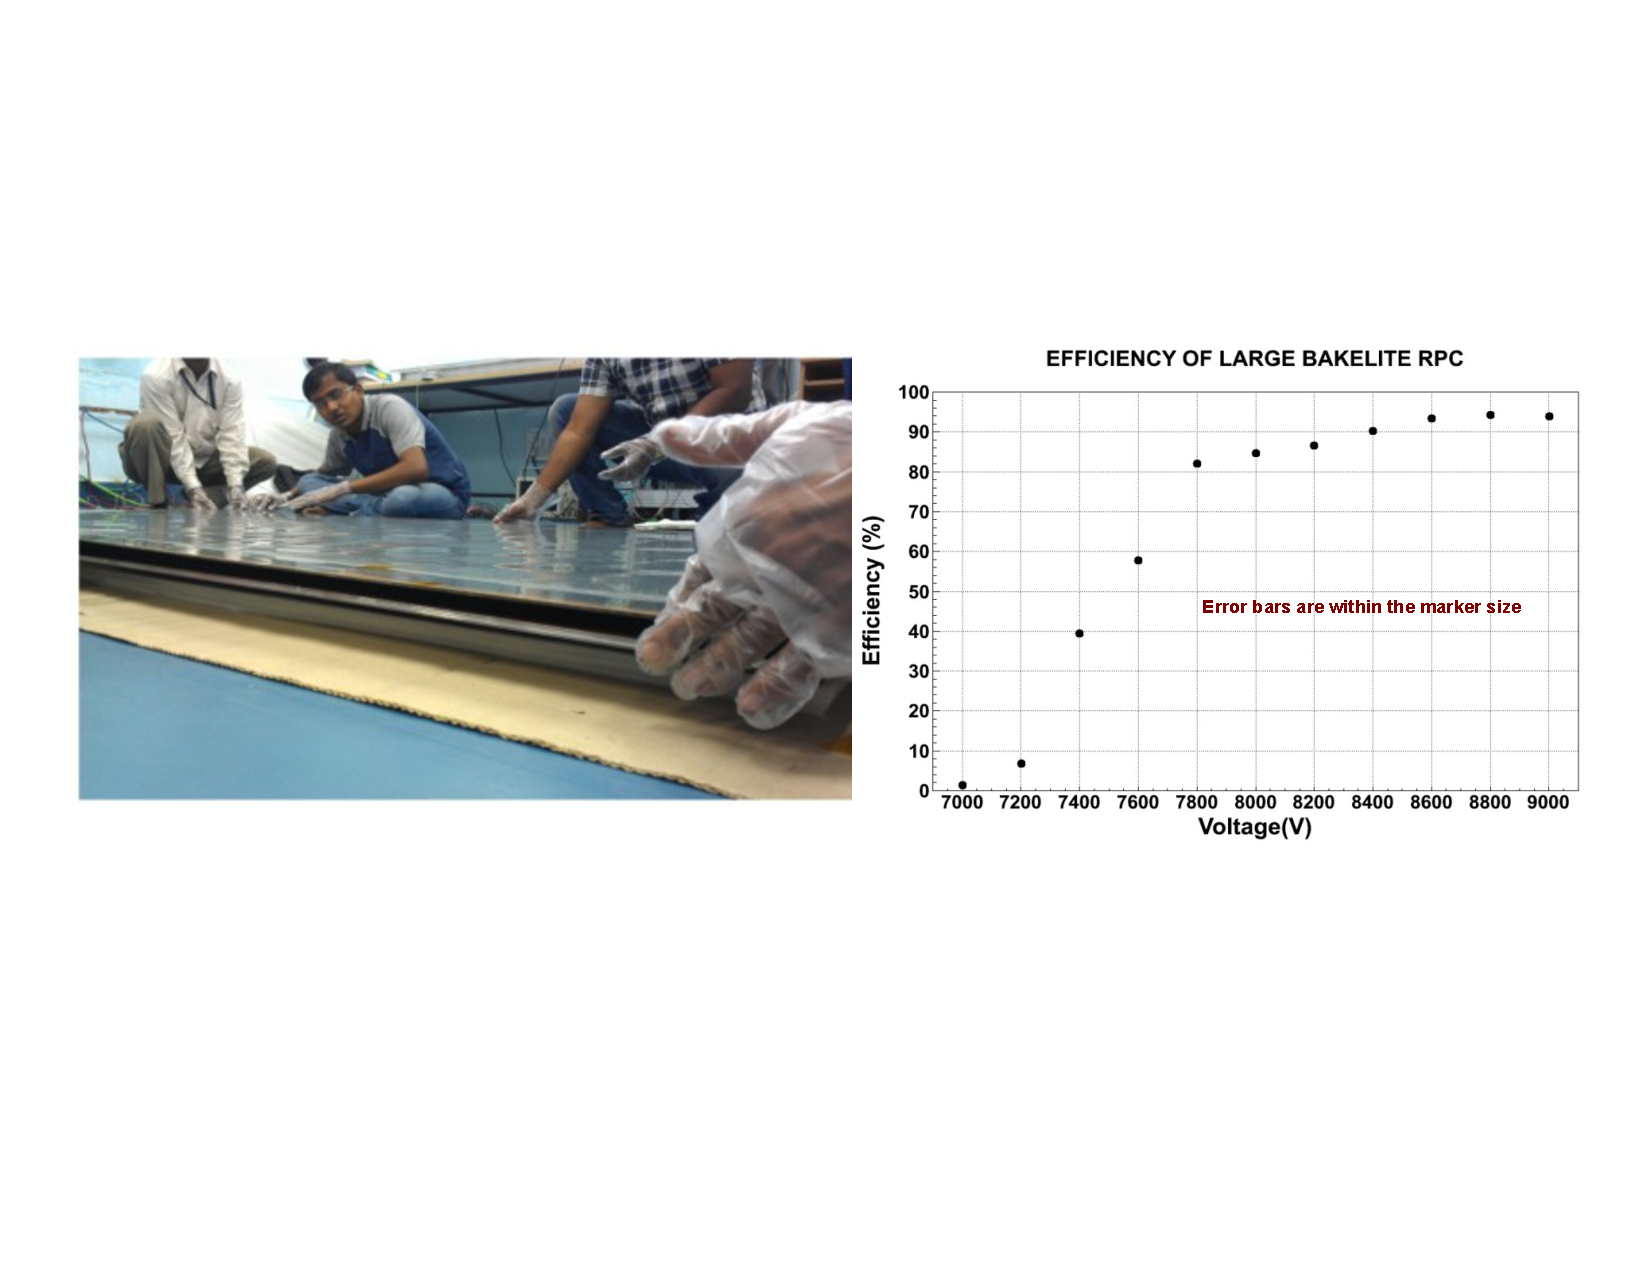
\includegraphics[width=\textwidth]{RPC_Prototype} % [width=5in,angle=90] <-- was too small
\end{cdrfigure}



%%%%%%%%%%%%%%%%%e
\subsection{Instrumentation}
\label{cdrsec:detectors-nd-ref-fgt-instrum}

The instrumentation includes both fast readout electronics for the
subdetectors and slow control of the subdetectors, involving
monitoring the humidity, temperature, gas pressure, etc.  There is
considerable synergy in the information gathered in the STT, ECAL and
MuID.  Both the STT and ECAL are required to measure the total charge
and the time associated with a given hit. The MuID RPCs are required
to provide the position and time associated with a traversing
track. Similarly, the slow control of the subdetectors share many
features.

The electronics for the three subsystems, STT, MuID, and ECAL, are all
``fast'' systems, i.e., all of the signals are in the few-to-10
nanosecond range.  The requirements for each system are very similar:
a fast output and both an ADC and a TDC on each channel.
Additionally, for the STT straw tubes it is desirable to wave-form
digitize the analog signal in order to enhance the ability to separate
the ionization signal from the transition radiation signal.  The total
channel count in FGT is 433,152 channels, as shown in
Table~\ref{tab:elect_ch}.
\begin{cdrtable}[Number of electronics channels for each of the
three detector systems]{ll}{elect_ch}{The number of electronics channels for each of the
three detector systems}
Detector&\# of Channels\\ \toprowrule
STT & 215,040 \\  \colhline
ECAL & 52,224 \\  \colhline
MuID & 165,888 \\
\end{cdrtable}

Recently, an interesting new ASIC development for an upgrade to the
ATLAS muon system at the LHC has come out of BNL), the VMM2 chip.
%\fixme{add G. DeGeronimo at BNL ref} 
It handles 64 channels and produces both fast ADC and TDC outputs.  It
has been fabricated and tested and should be ready by 2017, long
before it will be needed for DUNE.

To maintain a low level of humidity and to maintain a desired
temperature, both STT and ECAL subdetectors will have dry nitrogen
circulating within their outer layers.  Magnet coils are cooled by
water, while the magnet yokes are instrumented with RPCs that must
remain dry. Continuous control of humidity in all these detectors is
needed.  Temperature must also be continuously monitored in all of the
subdetectors in order for the electronics to not overheat.
%To ensure that the magnet does not overheat, the water flow (pressure gradient) will be continuously monitored.  
Also, all power sources instrumenting the FGT and its readout need to be monitored for 
appropriate voltage and current.

Gas leaks need to be monitored in the STT and MuID.  The STT will
employ Xe gas, which helps with the measurement of transition
radiation.  Xe gas is expensive and, hence, will be recirculated;
leak-monitoring is particularly important here.  The requirement on
leaks is less stringent for the RPCs, which have less expensive gas.

The water flow (pressure gradient) will be continuously monitored in
order to ensure that the magnet does not overheat.

